\documentclass[UTF8,11pt]{ctexart}
\usepackage[a4paper,margin=22mm]{geometry}
\usepackage{amsmath,amssymb,bm,graphicx,adjustbox,fvextra,longtable,array}
\xeCJKDeclareCharClass{CJK}{"2160 -> "217F, "2460 -> "249B, "2200 -> "22FF}
\newcommand{\fitmath}[1]{\begin{adjustbox}{max width=\linewidth}$\displaystyle #1$\end{adjustbox}}
\setlength{\parindent}{0pt}\setlength{\parskip}{.65em}\renewcommand{\arraystretch}{1.3}
\sloppy\allowdisplaybreaks
\begin{document}
\section*{2025 年计算机统考 408 · 真题}
\subsection*{2025年全国硕士研究生入学统一考试}

\subsection*{计算机学科专业基础综合试题}

\subsection*{一、单项选择题（1～40小题，每小题2分，共80分。下列每小题给出的四个选项中，只有一项符合题目要求）}

1．下列程序段的时间复杂度是\_\_\_\_\_\_。


\begin{Verbatim}[breaklines,breakanywhere,fontsize=\small]
int count=0, i, j;
for(i=1; i*i<=n; i++)
  for(j=1; j<=i; j++)
    count ++;
\end{Verbatim}

\begin{center}\begin{tabular}{>{\raggedright\arraybackslash}p{\dimexpr(\linewidth-8\tabcolsep)/4\relax}>{\raggedright\arraybackslash}p{\dimexpr(\linewidth-8\tabcolsep)/4\relax}>{\raggedright\arraybackslash}p{\dimexpr(\linewidth-8\tabcolsep)/4\relax}>{\raggedright\arraybackslash}p{\dimexpr(\linewidth-8\tabcolsep)/4\relax}}
\textbf{A.} \(\displaystyle O(\log n)\) & \textbf{B.} \(\displaystyle O(n)\) & \textbf{C.} \(\displaystyle O(n\log n)\) & \textbf{D.} \(\displaystyle O(n^2)\)\\[.35em]\end{tabular}\end{center}

2．已知算法A用于检查字符串中各类括号是否匹配，A执行过程中使用初始为空的栈保存遇到的括号。若栈的容量是3，则下列选项中，A不能处理的是\_\_\_\_\_\_。


\begin{center}\begin{tabular}{>{\raggedright\arraybackslash}p{\dimexpr(\linewidth-4\tabcolsep)/2\relax}>{\raggedright\arraybackslash}p{\dimexpr(\linewidth-4\tabcolsep)/2\relax}}
\textbf{A.} (a + [b + (c + d) / e] + f) + g – h & \textbf{B.} [a * ((b + c) / (d – e) + f / g) - h]\\[.35em]
\textbf{C.} [a * (b – (c – d) * e / (f + g)) – h] & \textbf{D.} [a – (b + [c * (d + e) – f] + g + h)]\\[.35em]\end{tabular}\end{center}

3．若二叉树的结点值均为正整数，采用顺序存储方式保存在数组R中，用－1表示结点不存在，则下列数组中，不能表示一棵二叉树的是\_\_\_\_\_\_。


\begin{center}\begin{tabular}{>{\raggedright\arraybackslash}p{\dimexpr(\linewidth-4\tabcolsep)/2\relax}>{\raggedright\arraybackslash}p{\dimexpr(\linewidth-4\tabcolsep)/2\relax}}
\textbf{A.} R[]=\{20, 15, 40, －1, －1, 35\} & \textbf{B.} R[]=\{15, 40, 10, 18, 35, －1, －1\}\\[.35em]
\textbf{C.} R[]=\{15, 40, 10, －1, －1, －1, 12\} & \textbf{D.} R[]=\{17, 20, 35, －1, 18, 45, －1, －1, 19, 27\}\\[.35em]\end{tabular}\end{center}

4．下列关于二叉树及森林的叙述中，正确的是：


\begin{center}\begin{tabular}{>{\raggedright\arraybackslash}p{\dimexpr(\linewidth-4\tabcolsep)/2\relax}>{\raggedright\arraybackslash}p{\dimexpr(\linewidth-4\tabcolsep)/2\relax}}
\textbf{A.} 完全二叉树中不存在度为1 的结点 & \textbf{B.} 任意一个森林都可以转换为一棵二叉树\\[.35em]
\textbf{C.} 二叉树的分支结点个数比叶结点个数少 & \textbf{D.} 表达式树的根中保存的是最先计算的运算符\\[.35em]\end{tabular}\end{center}

5．设字符集S 包含7 个字符，各字符出现的频次分别为2, 3, 4, 6, 8, 10, 11。现为S 中的各字符构造哈夫曼编码，编码长度不小于3 的字符个数是\_\_\_\_\_\_。


\begin{center}\begin{tabular}{>{\raggedright\arraybackslash}p{\dimexpr(\linewidth-8\tabcolsep)/4\relax}>{\raggedright\arraybackslash}p{\dimexpr(\linewidth-8\tabcolsep)/4\relax}>{\raggedright\arraybackslash}p{\dimexpr(\linewidth-8\tabcolsep)/4\relax}>{\raggedright\arraybackslash}p{\dimexpr(\linewidth-8\tabcolsep)/4\relax}}
\textbf{A.} 2 & \textbf{B.} 3 & \textbf{C.} 4 & \textbf{D.} 5\\[.35em]\end{tabular}\end{center}

6．下列关于图的叙述中，正确的是\_\_\_\_\_\_。


\begin{center}\begin{tabular}{>{\raggedright\arraybackslash}p{\dimexpr(\linewidth-4\tabcolsep)/2\relax}>{\raggedright\arraybackslash}p{\dimexpr(\linewidth-4\tabcolsep)/2\relax}}
\textbf{A.} 有向图必存在入度为0 的顶点 & \textbf{B.} 有向无环图的拓扑有序序列存在且唯一\\[.35em]
\textbf{C.} 各顶点的度均大于等于2 的无向图必有回路 & \textbf{D.} 可用 BFS 算法求出带权图中每一对顶点间的最短路径\\[.35em]\end{tabular}\end{center}

7．已知查找表中有400 个元素，查找每个元素的概率相同。采用分块查找法进行查找，且均匀分块。 若采用顺序查找法确定元素所在的块，且块内也采用顺序查找法，为使查找效率最高，则每块包含的元素个数应为\_\_\_\_\_\_。


\begin{center}\begin{tabular}{>{\raggedright\arraybackslash}p{\dimexpr(\linewidth-8\tabcolsep)/4\relax}>{\raggedright\arraybackslash}p{\dimexpr(\linewidth-8\tabcolsep)/4\relax}>{\raggedright\arraybackslash}p{\dimexpr(\linewidth-8\tabcolsep)/4\relax}>{\raggedright\arraybackslash}p{\dimexpr(\linewidth-8\tabcolsep)/4\relax}}
\textbf{A.} 8 & \textbf{B.} 10 & \textbf{C.} 20 & \textbf{D.} 25\\[.35em]\end{tabular}\end{center}

8．给定7 个不同的关键字，能够构造的不同4 阶B 树的个数最多是\_\_\_\_\_\_。


\begin{center}\begin{tabular}{>{\raggedright\arraybackslash}p{\dimexpr(\linewidth-8\tabcolsep)/4\relax}>{\raggedright\arraybackslash}p{\dimexpr(\linewidth-8\tabcolsep)/4\relax}>{\raggedright\arraybackslash}p{\dimexpr(\linewidth-8\tabcolsep)/4\relax}>{\raggedright\arraybackslash}p{\dimexpr(\linewidth-8\tabcolsep)/4\relax}}
\textbf{A.} 7 & \textbf{B.} 8 & \textbf{C.} 9 & \textbf{D.} 10\\[.35em]\end{tabular}\end{center}

9．下列关于散列方法处理冲突的叙述中，正确的是\_\_\_\_\_\_。


\begin{center}\begin{tabular}{>{\raggedright\arraybackslash}p{\dimexpr(\linewidth-4\tabcolsep)/2\relax}>{\raggedright\arraybackslash}p{\dimexpr(\linewidth-4\tabcolsep)/2\relax}}
\textbf{A.} 只要散列表不满，线性探查再散列一定能找到一个空闲位置 & \textbf{B.} 只要散列表不满，二次探查再散列一定能找到一个空闲位置\\[.35em]
\textbf{C.} 线性探查再散列处理的冲突，一定是发生在同义词之间的冲突 & \textbf{D.} 二次探查再散列处理的冲突，一定是发生在非同义词之间的冲突\\[.35em]\end{tabular}\end{center}

10．下列排序算法中，最坏情况下元素移动次数最少的是\_\_\_\_\_\_。


\begin{center}\begin{tabular}{>{\raggedright\arraybackslash}p{\dimexpr(\linewidth-8\tabcolsep)/4\relax}>{\raggedright\arraybackslash}p{\dimexpr(\linewidth-8\tabcolsep)/4\relax}>{\raggedright\arraybackslash}p{\dimexpr(\linewidth-8\tabcolsep)/4\relax}>{\raggedright\arraybackslash}p{\dimexpr(\linewidth-8\tabcolsep)/4\relax}}
\textbf{A.} 起泡排序 & \textbf{B.} 直接插入排序 & \textbf{C.} 快速排序 & \textbf{D.} 简单选择排序\\[.35em]\end{tabular}\end{center}

11．对含9个关键字的初始序列进行排序，若序列的变化情况如下表所示，则下列排序算法中，采用的是\_\_\_\_\_\_。


\begin{center}\begin{adjustbox}{max width=\linewidth}\begin{tabular}{|>{\raggedright\arraybackslash}p{\dimexpr(\linewidth-4\tabcolsep-3\arrayrulewidth)/2\relax}|>{\raggedright\arraybackslash}p{\dimexpr(\linewidth-4\tabcolsep-3\arrayrulewidth)/2\relax}|}\hline
初始序列 & 5, 25, 40, 30, 10, 20, 45, 15, 35\\\hline
第1趟排序后的序列 & 5, 10, 20, 30, 15, 35, 45, 25, 40\\\hline
第2趟排序后的序列 & 5, 10, 15, 25, 20, 30, 40, 35, 45\\\hline\end{tabular}\end{adjustbox}\end{center}

\begin{center}\begin{tabular}{>{\raggedright\arraybackslash}p{\dimexpr(\linewidth-8\tabcolsep)/4\relax}>{\raggedright\arraybackslash}p{\dimexpr(\linewidth-8\tabcolsep)/4\relax}>{\raggedright\arraybackslash}p{\dimexpr(\linewidth-8\tabcolsep)/4\relax}>{\raggedright\arraybackslash}p{\dimexpr(\linewidth-8\tabcolsep)/4\relax}}
\textbf{A.} 希尔排序 & \textbf{B.} 基数排序 & \textbf{C.} 归并排序 & \textbf{D.} 折半插入排序\\[.35em]\end{tabular}\end{center}

12．在32位计算机上执行下列C语言代码段后，ui的值是\_\_\_\_\_\_。


\begin{Verbatim}[breaklines,breakanywhere,fontsize=\small]
short si=-32767;
unsigned int ui=si;
\end{Verbatim}

\begin{center}\begin{tabular}{>{\raggedright\arraybackslash}p{\dimexpr(\linewidth-8\tabcolsep)/4\relax}>{\raggedright\arraybackslash}p{\dimexpr(\linewidth-8\tabcolsep)/4\relax}>{\raggedright\arraybackslash}p{\dimexpr(\linewidth-8\tabcolsep)/4\relax}>{\raggedright\arraybackslash}p{\dimexpr(\linewidth-8\tabcolsep)/4\relax}}
\textbf{A.} \(\displaystyle 2^{15}-1\) & \textbf{B.} \(\displaystyle 2^{15}+1\) & \textbf{C.} \(\displaystyle 2^{32}-2^{15}-1\) & \textbf{D.} \(\displaystyle 2^{32}-2^{15}+1\)\\[.35em]\end{tabular}\end{center}

13．已知float型变量用IEEE 754单精度浮点数格式表示。若float型变量x的机器数为4730 0000H，则x的值是\_\_\_\_\_\_。


\begin{center}\begin{tabular}{>{\raggedright\arraybackslash}p{\dimexpr(\linewidth-8\tabcolsep)/4\relax}>{\raggedright\arraybackslash}p{\dimexpr(\linewidth-8\tabcolsep)/4\relax}>{\raggedright\arraybackslash}p{\dimexpr(\linewidth-8\tabcolsep)/4\relax}>{\raggedright\arraybackslash}p{\dimexpr(\linewidth-8\tabcolsep)/4\relax}}
\textbf{A.} \(\displaystyle 0.375\times2^{14}\) & \textbf{B.} \(\displaystyle 1.375\times2^{14}\) & \textbf{C.} \(\displaystyle 0.375\times2^{15}\) & \textbf{D.} \(\displaystyle 1.375\times2^{15}\)\\[.35em]\end{tabular}\end{center}

14．假设8位字长的计算机中，两个带符号整数x和y的补码表示分别为\(\displaystyle [x]_{\text{补}}=\mathrm{A3H}\)、\(\displaystyle [y]_{\text{补}}=\mathrm{75H}\)，则通过补码加减运算器得到的\(\displaystyle x-y\)的值及OF标志分别为\_\_\_\_\_\_。


\begin{center}\begin{tabular}{>{\raggedright\arraybackslash}p{\dimexpr(\linewidth-8\tabcolsep)/4\relax}>{\raggedright\arraybackslash}p{\dimexpr(\linewidth-8\tabcolsep)/4\relax}>{\raggedright\arraybackslash}p{\dimexpr(\linewidth-8\tabcolsep)/4\relax}>{\raggedright\arraybackslash}p{\dimexpr(\linewidth-8\tabcolsep)/4\relax}}
\textbf{A.} 24, 0 & \textbf{B.} 24, 1 & \textbf{C.} 46, 0 & \textbf{D.} 46, 1\\[.35em]\end{tabular}\end{center}

15．某32位计算机按字节编址，采用小端方式存放数据，编译器按边界对齐方式为下列C语言结构型数组变量employee分配存储空间。


\begin{Verbatim}[breaklines,breakanywhere,fontsize=\small]
struct record{
  int id;
  char name[10];
  int salary;
} employee[200];
\end{Verbatim}

若employee的首地址为0000 A0B0H，employee[1].id的机器数为1234 5678H，则该机器数中的56H所在存储单元的地址是\_\_\_\_\_\_。


\begin{center}\begin{tabular}{>{\raggedright\arraybackslash}p{\dimexpr(\linewidth-8\tabcolsep)/4\relax}>{\raggedright\arraybackslash}p{\dimexpr(\linewidth-8\tabcolsep)/4\relax}>{\raggedright\arraybackslash}p{\dimexpr(\linewidth-8\tabcolsep)/4\relax}>{\raggedright\arraybackslash}p{\dimexpr(\linewidth-8\tabcolsep)/4\relax}}
\textbf{A.} 0000 A0C3H & \textbf{B.} 0000 A0C4H & \textbf{C.} 0000 A0C5H & \textbf{D.} 0000 A0C6H\\[.35em]\end{tabular}\end{center}

16．下列选项中，由指令集体系结构（ISA）规定的是\_\_\_\_\_\_。


\begin{center}\begin{tabular}{>{\raggedright\arraybackslash}p{\dimexpr(\linewidth-4\tabcolsep)/2\relax}>{\raggedright\arraybackslash}p{\dimexpr(\linewidth-4\tabcolsep)/2\relax}}
\textbf{A.} 是否采用阵列乘法器 & \textbf{B.} 是否采用定长指令字格式\\[.35em]
\textbf{C.} 是否采用微程序控制器 & \textbf{D.} 是否采用单总线数据通路\\[.35em]\end{tabular}\end{center}

17．下列关于RISC 的叙述中，错误的是：


\begin{center}\begin{tabular}{>{\raggedright\arraybackslash}p{\dimexpr(\linewidth-4\tabcolsep)/2\relax}>{\raggedright\arraybackslash}p{\dimexpr(\linewidth-4\tabcolsep)/2\relax}}
\textbf{A.} 多采用硬连线方式实现控制器 & \textbf{B.} 通常采用 Load/Store 型指令设计风格\\[.35em]
\textbf{C.} 难以采用流水线数据通路实现微架构 & \textbf{D.} 多采用寄存器传递过程调用时的参数\\[.35em]\end{tabular}\end{center}

18．下列关于CPI 和CPU 时钟周期的叙述中，错误的是：


\begin{center}\begin{tabular}{>{\raggedright\arraybackslash}p{\dimexpr(\linewidth-4\tabcolsep)/2\relax}>{\raggedright\arraybackslash}p{\dimexpr(\linewidth-4\tabcolsep)/2\relax}}
\textbf{A.} 不同类型指令的CPI 可能不一样 & \textbf{B.} 程序的CPI 与Cache 缺失率无关\\[.35em]
\textbf{C.} 单周期CPU 的时钟周期以最耗时指令所用时间为准 & \textbf{D.} 流水线CPU 的时钟周期以最长流水段所用时间为准\\[.35em]\end{tabular}\end{center}

19．下列关于CPU 中的数据通路和控制器的叙述中，错误的是：


\begin{center}\begin{tabular}{>{\raggedright\arraybackslash}p{\dimexpr(\linewidth-4\tabcolsep)/2\relax}>{\raggedright\arraybackslash}p{\dimexpr(\linewidth-4\tabcolsep)/2\relax}}
\textbf{A.} 通用寄存器组中应该包含程序计数器 & \textbf{B.} 控制器中一定包含指令操作码的译码电路\\[.35em]
\textbf{C.} 单周期CPU 中的控制器比多周期CPU 中的更简单 & \textbf{D.} 流水线CPU 需解决数据相关和控制相关等冒险问题\\[.35em]\end{tabular}\end{center}

20．某处理器总线采用同步、并行传输方式，每个总线时钟周期传送4次数据（quadpumped技术）。若该总线的工作频率为1333MHz（实际单位是MT/s，表示每秒传送1333M次），总线宽度为64位，则总线带宽约为\_\_\_\_\_\_。


\begin{center}\begin{tabular}{>{\raggedright\arraybackslash}p{\dimexpr(\linewidth-8\tabcolsep)/4\relax}>{\raggedright\arraybackslash}p{\dimexpr(\linewidth-8\tabcolsep)/4\relax}>{\raggedright\arraybackslash}p{\dimexpr(\linewidth-8\tabcolsep)/4\relax}>{\raggedright\arraybackslash}p{\dimexpr(\linewidth-8\tabcolsep)/4\relax}}
\textbf{A.} 10.\allowbreak{}66 GB/s & \textbf{B.} 42.\allowbreak{}66 GB/s & \textbf{C.} 85.\allowbreak{}31 GB/s & \textbf{D.} 341.\allowbreak{}25 GB/s\\[.35em]\end{tabular}\end{center}

21．下列设备中，适合采用DMA 输入/输出方式的是\_\_\_\_\_\_。 I. 键盘 II. 网卡 III. 固态硬盘 IV. 针式打印机


\begin{center}\begin{tabular}{>{\raggedright\arraybackslash}p{\dimexpr(\linewidth-8\tabcolsep)/4\relax}>{\raggedright\arraybackslash}p{\dimexpr(\linewidth-8\tabcolsep)/4\relax}>{\raggedright\arraybackslash}p{\dimexpr(\linewidth-8\tabcolsep)/4\relax}>{\raggedright\arraybackslash}p{\dimexpr(\linewidth-8\tabcolsep)/4\relax}}
\textbf{A.} 仅I、II & \textbf{B.} 仅II、III & \textbf{C.} 仅II、IV & \textbf{D.} 仅III、IV\\[.35em]\end{tabular}\end{center}

22．下列选项中，会触发外部中断请求的事件是\_\_\_\_\_\_。


\begin{center}\begin{tabular}{>{\raggedright\arraybackslash}p{\dimexpr(\linewidth-8\tabcolsep)/4\relax}>{\raggedright\arraybackslash}p{\dimexpr(\linewidth-8\tabcolsep)/4\relax}>{\raggedright\arraybackslash}p{\dimexpr(\linewidth-8\tabcolsep)/4\relax}>{\raggedright\arraybackslash}p{\dimexpr(\linewidth-8\tabcolsep)/4\relax}}
\textbf{A.} DMA 传送结束 & \textbf{B.} 总线事务结束 & \textbf{C.} 页故障处理结束 & \textbf{D.} 执行断点指令\\[.35em]\end{tabular}\end{center}

23．在采用页式虚拟存储管理方式的系统中，当发生进程上下文切换时，下列寄存器中，操作系统不需要更新的是\_\_\_\_\_\_。


\begin{center}\begin{tabular}{>{\raggedright\arraybackslash}p{\dimexpr(\linewidth-4\tabcolsep)/2\relax}>{\raggedright\arraybackslash}p{\dimexpr(\linewidth-4\tabcolsep)/2\relax}}
\textbf{A.} 通用寄存器 & \textbf{B.} 页表基址寄存器\\[.35em]
\textbf{C.} 程序计数器 & \textbf{D.} 内核中断向量表基址寄存器\\[.35em]\end{tabular}\end{center}

24．下列关于虚拟化技术的叙述中，错误的是\_\_\_\_\_\_。


\begin{center}\begin{tabular}{>{\raggedright\arraybackslash}p{\dimexpr(\linewidth-4\tabcolsep)/2\relax}>{\raggedright\arraybackslash}p{\dimexpr(\linewidth-4\tabcolsep)/2\relax}}
\textbf{A.} 操作系统可以运行在虚拟机上 & \textbf{B.} 虚拟化技术支持在一台计算机上构建多个虚拟机\\[.35em]
\textbf{C.} 虚拟机监控程序（VMM）与操作系统的特权级相同 & \textbf{D.} 虚拟化技术支持在一台计算机上模拟不同的指令集体系结构\\[.35em]\end{tabular}\end{center}

25．某基于优先权的进程调度程序中，进程就绪队列采用优先权由高到低的有序单链表实现。若就绪队列长度为\(\displaystyle n\)，则就绪队列的插入操作和从就绪队列中选出将要执行进程的操作的时间复杂度分别是\_\_\_\_\_\_。


\begin{center}\begin{tabular}{>{\raggedright\arraybackslash}p{\dimexpr(\linewidth-8\tabcolsep)/4\relax}>{\raggedright\arraybackslash}p{\dimexpr(\linewidth-8\tabcolsep)/4\relax}>{\raggedright\arraybackslash}p{\dimexpr(\linewidth-8\tabcolsep)/4\relax}>{\raggedright\arraybackslash}p{\dimexpr(\linewidth-8\tabcolsep)/4\relax}}
\textbf{A.} \(\displaystyle O(1),\allowbreak O(1)\) & \textbf{B.} \(\displaystyle O(1),\allowbreak O(n)\) & \textbf{C.} \(\displaystyle O(n),\allowbreak O(1)\) & \textbf{D.} \(\displaystyle O(n),\allowbreak O(n)\)\\[.35em]\end{tabular}\end{center}

26．某页式虚拟存储管理系统采用固定分配局部置换的LRU 算法。若系统为进程P 分配了3 个页框， P 从某时刻开始的页访问序列为0, 1, 2, 0, 5, 1, 4, 3, 0, 2, 3, 2, 0，且0, 1, 2 三个页已在内存中，则完成上述页序列的访问时，系统执行缺页异常处理程序的次数为\_\_\_\_\_\_。


\begin{center}\begin{tabular}{>{\raggedright\arraybackslash}p{\dimexpr(\linewidth-8\tabcolsep)/4\relax}>{\raggedright\arraybackslash}p{\dimexpr(\linewidth-8\tabcolsep)/4\relax}>{\raggedright\arraybackslash}p{\dimexpr(\linewidth-8\tabcolsep)/4\relax}>{\raggedright\arraybackslash}p{\dimexpr(\linewidth-8\tabcolsep)/4\relax}}
\textbf{A.} 5 & \textbf{B.} 6 & \textbf{C.} 7 & \textbf{D.} 8\\[.35em]\end{tabular}\end{center}

27．在页式虚拟存储管理系统中，确定进程正常运行所需的最少页框数时，下列因素中需要考虑的是\_\_\_\_\_\_。


\begin{center}\begin{tabular}{>{\raggedright\arraybackslash}p{\dimexpr(\linewidth-4\tabcolsep)/2\relax}>{\raggedright\arraybackslash}p{\dimexpr(\linewidth-4\tabcolsep)/2\relax}}
\textbf{A.} 代码段长度 & \textbf{B.} 进程的虚拟地址空间大小\\[.35em]
\textbf{C.} 物理内存大小 & \textbf{D.} 指令系统支持的寻址方式\\[.35em]\end{tabular}\end{center}

28．下列关于虚拟文件系统（VFS）的叙述中，正确的是\_\_\_\_\_\_。


\begin{center}\begin{tabular}{>{\raggedright\arraybackslash}p{\dimexpr(\linewidth-4\tabcolsep)/2\relax}>{\raggedright\arraybackslash}p{\dimexpr(\linewidth-4\tabcolsep)/2\relax}}
\textbf{A.} VFS 是在虚拟内存中建立的文件系统 & \textbf{B.} VFS 能提高不同文件系统中文件的访问速度\\[.35em]
\textbf{C.} VFS 定义了可以访问不同文件系统的统一接口 & \textbf{D.} 通过VFS 只能访问本地文件，不能访问网络文件\\[.35em]\end{tabular}\end{center}

29．某文件系统采用目录和索引节点管理文件，当用户在目录中新建文件F 时，下列操作中，文件系统不会做的是\_\_\_\_\_\_。


\begin{center}\begin{tabular}{>{\raggedright\arraybackslash}p{\dimexpr(\linewidth-4\tabcolsep)/2\relax}>{\raggedright\arraybackslash}p{\dimexpr(\linewidth-4\tabcolsep)/2\relax}}
\textbf{A.} 对F 的索引节点进行初始化 & \textbf{B.} 在目录文件中写入F 的索引节点号\\[.35em]
\textbf{C.} 在目录文件中写入F 的访问权限信息 & \textbf{D.} 在目录文件中增加一条F 对应的目录项\\[.35em]\end{tabular}\end{center}

30．下列关于内存映射文件（memory-mapped files）机制的叙述中，正确的是\_\_\_\_\_\_。 I. 可实现进程之间的通信 II. 可实现页到磁盘块的映射 III. 将文件映射到进程的虚拟地址空间 IV. 将文件映射到系统的物理地址空间


\begin{center}\begin{tabular}{>{\raggedright\arraybackslash}p{\dimexpr(\linewidth-8\tabcolsep)/4\relax}>{\raggedright\arraybackslash}p{\dimexpr(\linewidth-8\tabcolsep)/4\relax}>{\raggedright\arraybackslash}p{\dimexpr(\linewidth-8\tabcolsep)/4\relax}>{\raggedright\arraybackslash}p{\dimexpr(\linewidth-8\tabcolsep)/4\relax}}
\textbf{A.} 仅I、III & \textbf{B.} 仅I、IV & \textbf{C.} 仅II、III & \textbf{D.} 仅I、II、III\\[.35em]\end{tabular}\end{center}

31．下列选项中，文件系统可用于记录外存空闲空间使用情况的是\_\_\_\_\_\_。


\begin{center}\begin{tabular}{>{\raggedright\arraybackslash}p{\dimexpr(\linewidth-8\tabcolsep)/4\relax}>{\raggedright\arraybackslash}p{\dimexpr(\linewidth-8\tabcolsep)/4\relax}>{\raggedright\arraybackslash}p{\dimexpr(\linewidth-8\tabcolsep)/4\relax}>{\raggedright\arraybackslash}p{\dimexpr(\linewidth-8\tabcolsep)/4\relax}}
\textbf{A.} 目录 & \textbf{B.} 系统打开文件表 & \textbf{C.} 文件分配表（FAT） & \textbf{D.} 文件控制块（FCB）\\[.35em]\end{tabular}\end{center}

32．下列选项中，文件系统需要为温彻斯特硬盘和固态硬盘都提供的功能是\_\_\_\_\_\_。


\begin{center}\begin{tabular}{>{\raggedright\arraybackslash}p{\dimexpr(\linewidth-8\tabcolsep)/4\relax}>{\raggedright\arraybackslash}p{\dimexpr(\linewidth-8\tabcolsep)/4\relax}>{\raggedright\arraybackslash}p{\dimexpr(\linewidth-8\tabcolsep)/4\relax}>{\raggedright\arraybackslash}p{\dimexpr(\linewidth-8\tabcolsep)/4\relax}}
\textbf{A.} 划分扇区 & \textbf{B.} 确定盘块大小 & \textbf{C.} 降低寻道时间 & \textbf{D.} 实现均衡磨损\\[.35em]\end{tabular}\end{center}

33．某网络拓扑及各链路带宽如题33图所示。网络按电路交换方式运行时，主机H1与H2建立一条带宽为10Mb/s的电路，建立电路时间为\(\displaystyle 32\,\mu\mathrm{s}\)；按分组交换方式运行时，分组长度为400B，忽略分组首部开销。现H1向H2发送一个2MB（\(\displaystyle 1\mathrm{M}=10^6\)）的文件，分别采用电路交换、报文交换、分组交换方式时，H2至少需要\(\displaystyle T_{\mathrm{CS}}\)、\(\displaystyle T_{\mathrm{MS}}\)、\(\displaystyle T_{\mathrm{PS}}\)时间才能接收到全部文件内容，则\(\displaystyle T_{\mathrm{CS}}\)、\(\displaystyle T_{\mathrm{MS}}\)、\(\displaystyle T_{\mathrm{PS}}\)满足的关系是\_\_\_\_\_\_。


\begin{center}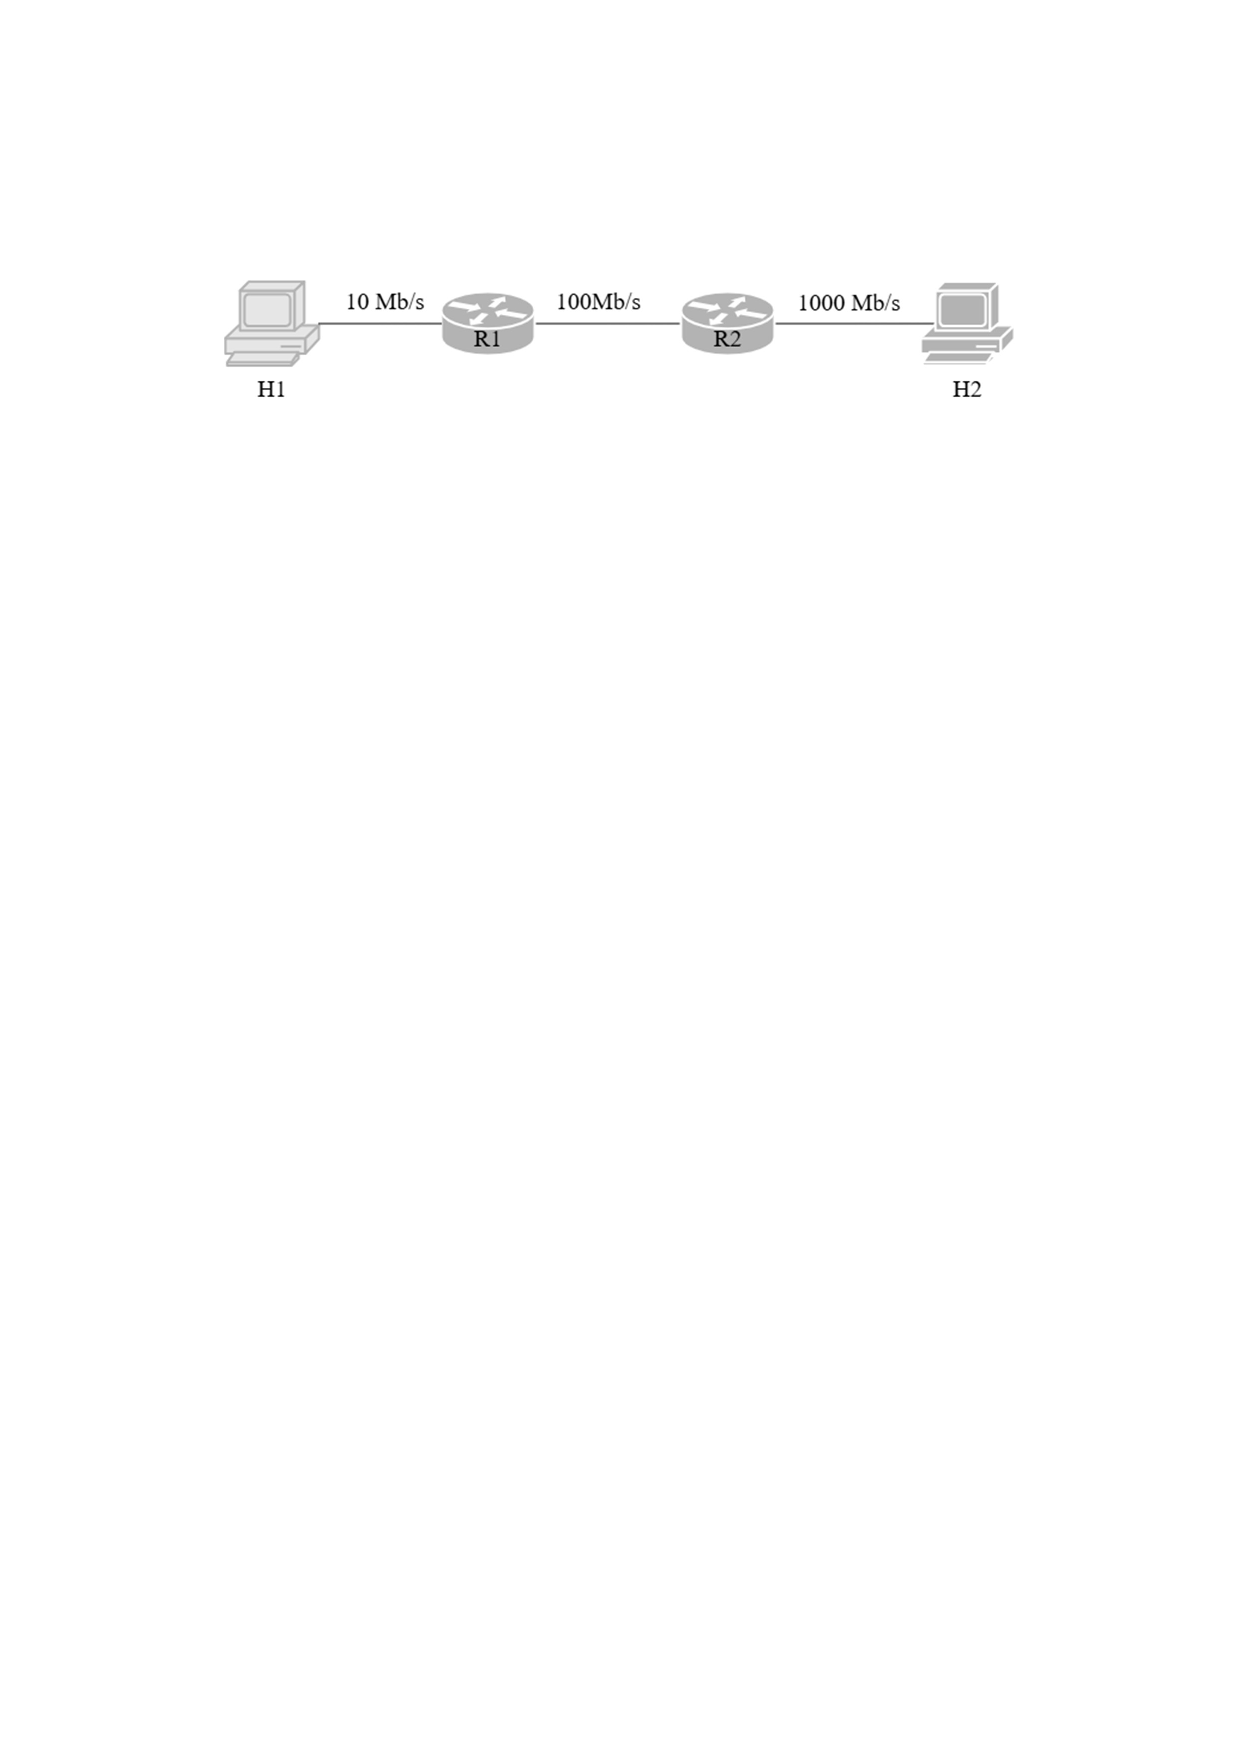
\includegraphics[width=.65\linewidth,height=.4\textheight,keepaspectratio]{../assets/figures/2025-questions-p004-b001.pdf}\end{center}

\begin{center}\begin{tabular}{>{\raggedright\arraybackslash}p{\dimexpr(\linewidth-4\tabcolsep)/2\relax}>{\raggedright\arraybackslash}p{\dimexpr(\linewidth-4\tabcolsep)/2\relax}}
\textbf{A.} \(\displaystyle T_{\mathrm{CS}}>T_{\mathrm{MS}}>T_{\mathrm{PS}}\) & \textbf{B.} \(\displaystyle T_{\mathrm{MS}}>T_{\mathrm{PS}}>T_{\mathrm{CS}}\)\\[.35em]
\textbf{C.} \(\displaystyle T_{\mathrm{MS}}>T_{\mathrm{CS}}>T_{\mathrm{PS}}\) & \textbf{D.} \(\displaystyle T_{\mathrm{PS}}>T_{\mathrm{MS}}>T_{\mathrm{CS}}\)\\[.35em]\end{tabular}\end{center}

34．若某差错编码的编码集为\{1001 1010, 0101 1100, 1111 0000, 0000 1111\}，则该差错编码的检错和纠错能力是：


\begin{center}\begin{tabular}{>{\raggedright\arraybackslash}p{\dimexpr(\linewidth-4\tabcolsep)/2\relax}>{\raggedright\arraybackslash}p{\dimexpr(\linewidth-4\tabcolsep)/2\relax}}
\textbf{A.} 不超过2 位错的100\%检错、不超过1 位错的纠错 & \textbf{B.} 不超过2 位错的100\%检错、不超过2 位错的纠错\\[.35em]
\textbf{C.} 不超过3 位错的100\%检错、不超过1 位错的纠错 & \textbf{D.} 不超过3 位错的100\%检错、不超过2 位错的纠错\\[.35em]\end{tabular}\end{center}

35．在某个10BaseT 以太网的冲突域内，若主机甲向主机乙发送数据帧时发生了连续11 次冲突，则甲再次尝试发送该数据帧的最大间隔时间是\_\_\_\_\_\_。


\begin{center}\begin{tabular}{>{\raggedright\arraybackslash}p{\dimexpr(\linewidth-8\tabcolsep)/4\relax}>{\raggedright\arraybackslash}p{\dimexpr(\linewidth-8\tabcolsep)/4\relax}>{\raggedright\arraybackslash}p{\dimexpr(\linewidth-8\tabcolsep)/4\relax}>{\raggedright\arraybackslash}p{\dimexpr(\linewidth-8\tabcolsep)/4\relax}}
\textbf{A.} 0.\allowbreak{}512ms & \textbf{B.} 0.\allowbreak{}5632ms & \textbf{C.} 52.\allowbreak{}3776ms & \textbf{D.} 104.\allowbreak{}8064ms\\[.35em]\end{tabular}\end{center}

36．一台新接入网络的主机H通过DHCP服务器动态请求IP地址过程中，与DHCP服务器交换DHCP报文的部分过程如题36图所示。封装DHCPREQUEST报文的IP数据报的目的IP地址和源IP地址分别是\_\_\_\_\_\_。


\begin{center}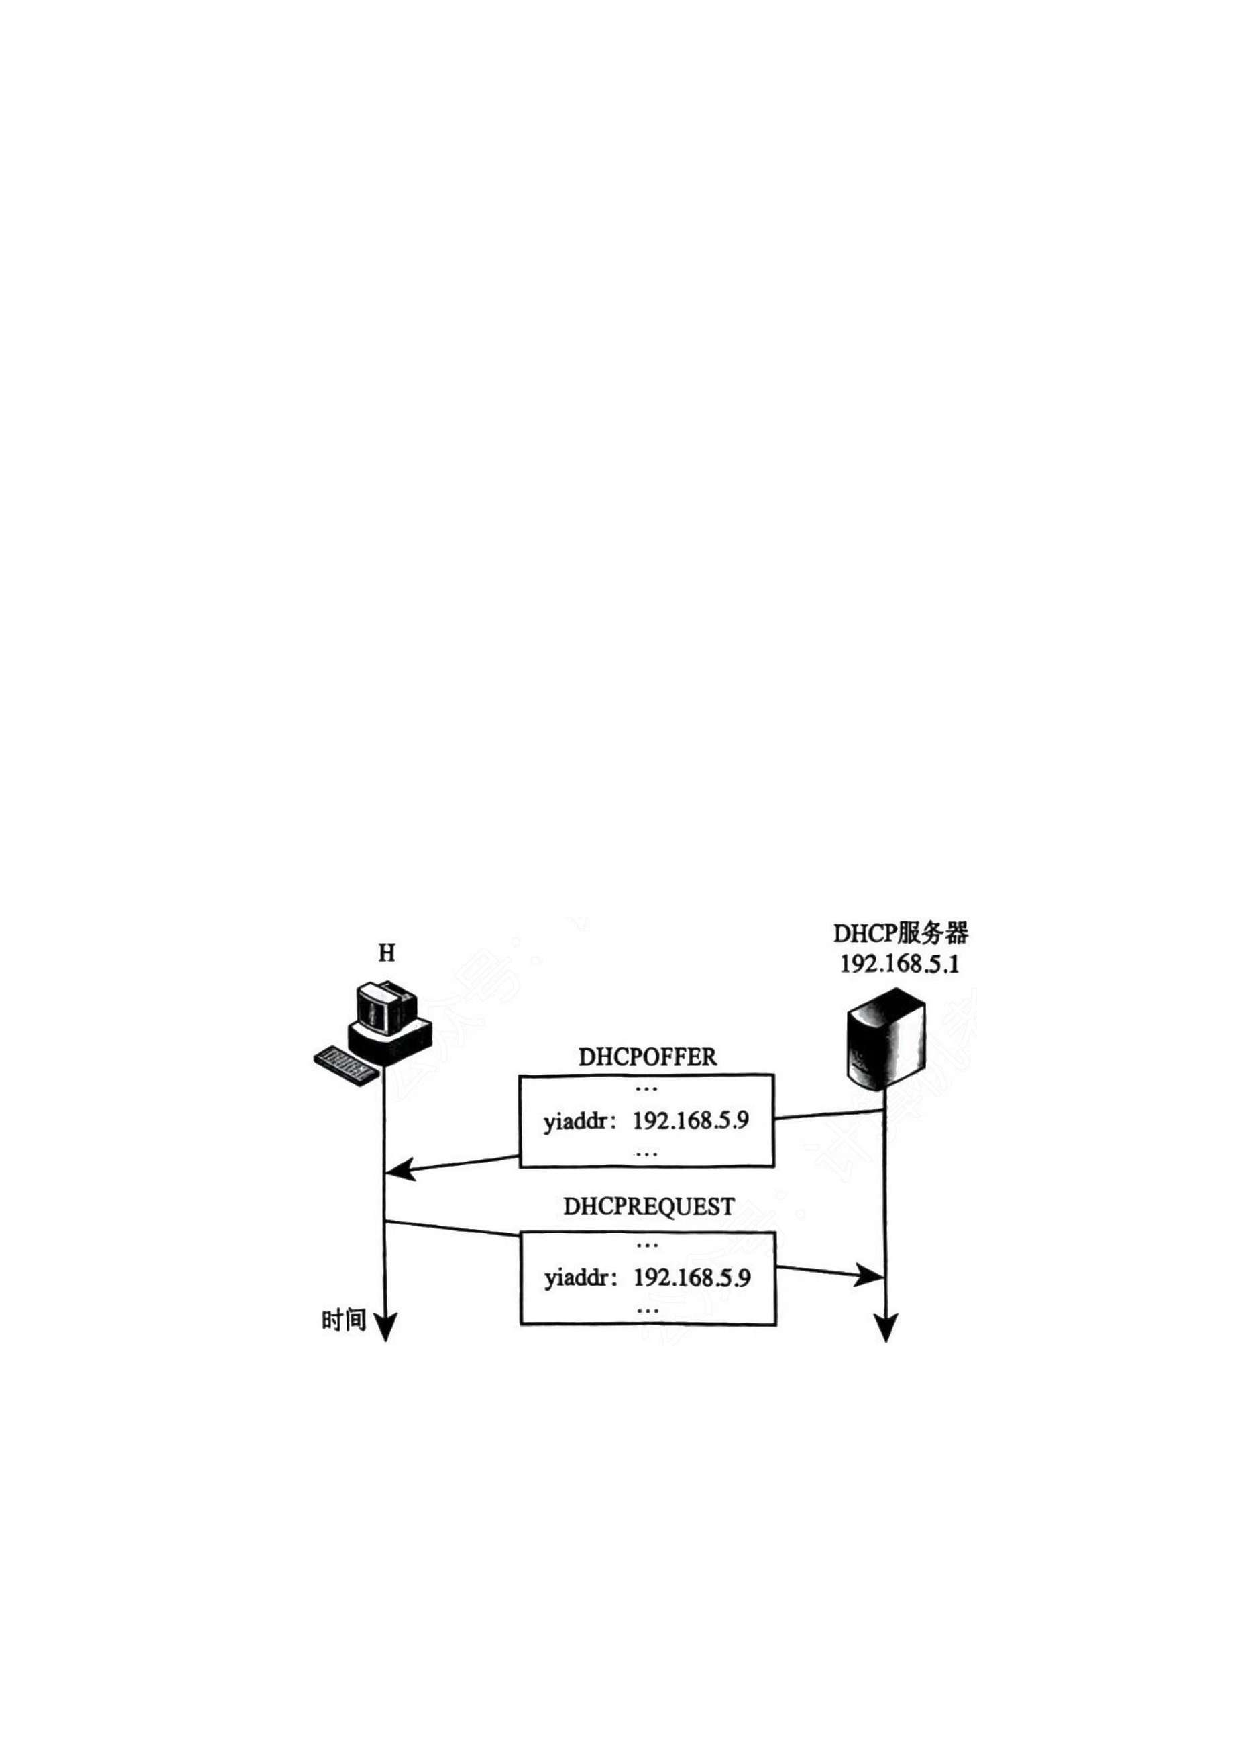
\includegraphics[width=.65\linewidth,height=.4\textheight,keepaspectratio]{../assets/figures/2025-questions-p004-b006.pdf}\end{center}

\begin{center}\begin{tabular}{>{\raggedright\arraybackslash}p{\dimexpr(\linewidth-4\tabcolsep)/2\relax}>{\raggedright\arraybackslash}p{\dimexpr(\linewidth-4\tabcolsep)/2\relax}}
\textbf{A.} 192.\allowbreak{}168.\allowbreak{}5.\allowbreak{}1, 0.\allowbreak{}0.\allowbreak{}0.\allowbreak{}0 & \textbf{B.} 192.\allowbreak{}168.\allowbreak{}5.\allowbreak{}1, 192.\allowbreak{}168.\allowbreak{}5.\allowbreak{}9\\[.35em]
\textbf{C.} 255.\allowbreak{}255.\allowbreak{}255.\allowbreak{}255, 0.\allowbreak{}0.\allowbreak{}0.\allowbreak{}0 & \textbf{D.} 255.\allowbreak{}255.\allowbreak{}255.\allowbreak{}255, 192.\allowbreak{}168.\allowbreak{}5.\allowbreak{}9\\[.35em]\end{tabular}\end{center}

37．假设路由器实现NAT 功能，内网中主机H 的IP 地址为192.168.1.5/24。若H 运行某应用向Internet 发送了一个UDP 报文段，则路由器在转发封装该UDP 报文段的IP 数据报的过程中，UDP 报文段的首部字段会被修改的是：I. 源端口号 II. 目的端口号 III. 总长度 IV. 校验和


\begin{center}\begin{tabular}{>{\raggedright\arraybackslash}p{\dimexpr(\linewidth-8\tabcolsep)/4\relax}>{\raggedright\arraybackslash}p{\dimexpr(\linewidth-8\tabcolsep)/4\relax}>{\raggedright\arraybackslash}p{\dimexpr(\linewidth-8\tabcolsep)/4\relax}>{\raggedright\arraybackslash}p{\dimexpr(\linewidth-8\tabcolsep)/4\relax}}
\textbf{A.} 仅I、III & \textbf{B.} 仅I、IV & \textbf{C.} 仅II、III & \textbf{D.} 仅II、IV\\[.35em]\end{tabular}\end{center}

38．主机甲通过TCP向主机乙发送数据的部分过程如题38图所示，seq为序号，ack\_seq为确认序号，rcvwnd为接收窗口。甲在\(\displaystyle t_0\)时刻的拥塞窗口和发送窗口均为2000B，拥塞控制值为8000B，MSS=1000B，甲始终以MSS发送TCP段。若甲在\(\displaystyle t_1\)时刻收到如图所示的确认段，则甲在未收到新的确认段之前，还可以继续向乙发送的TCP段数是\_\_\_\_\_\_。


\begin{center}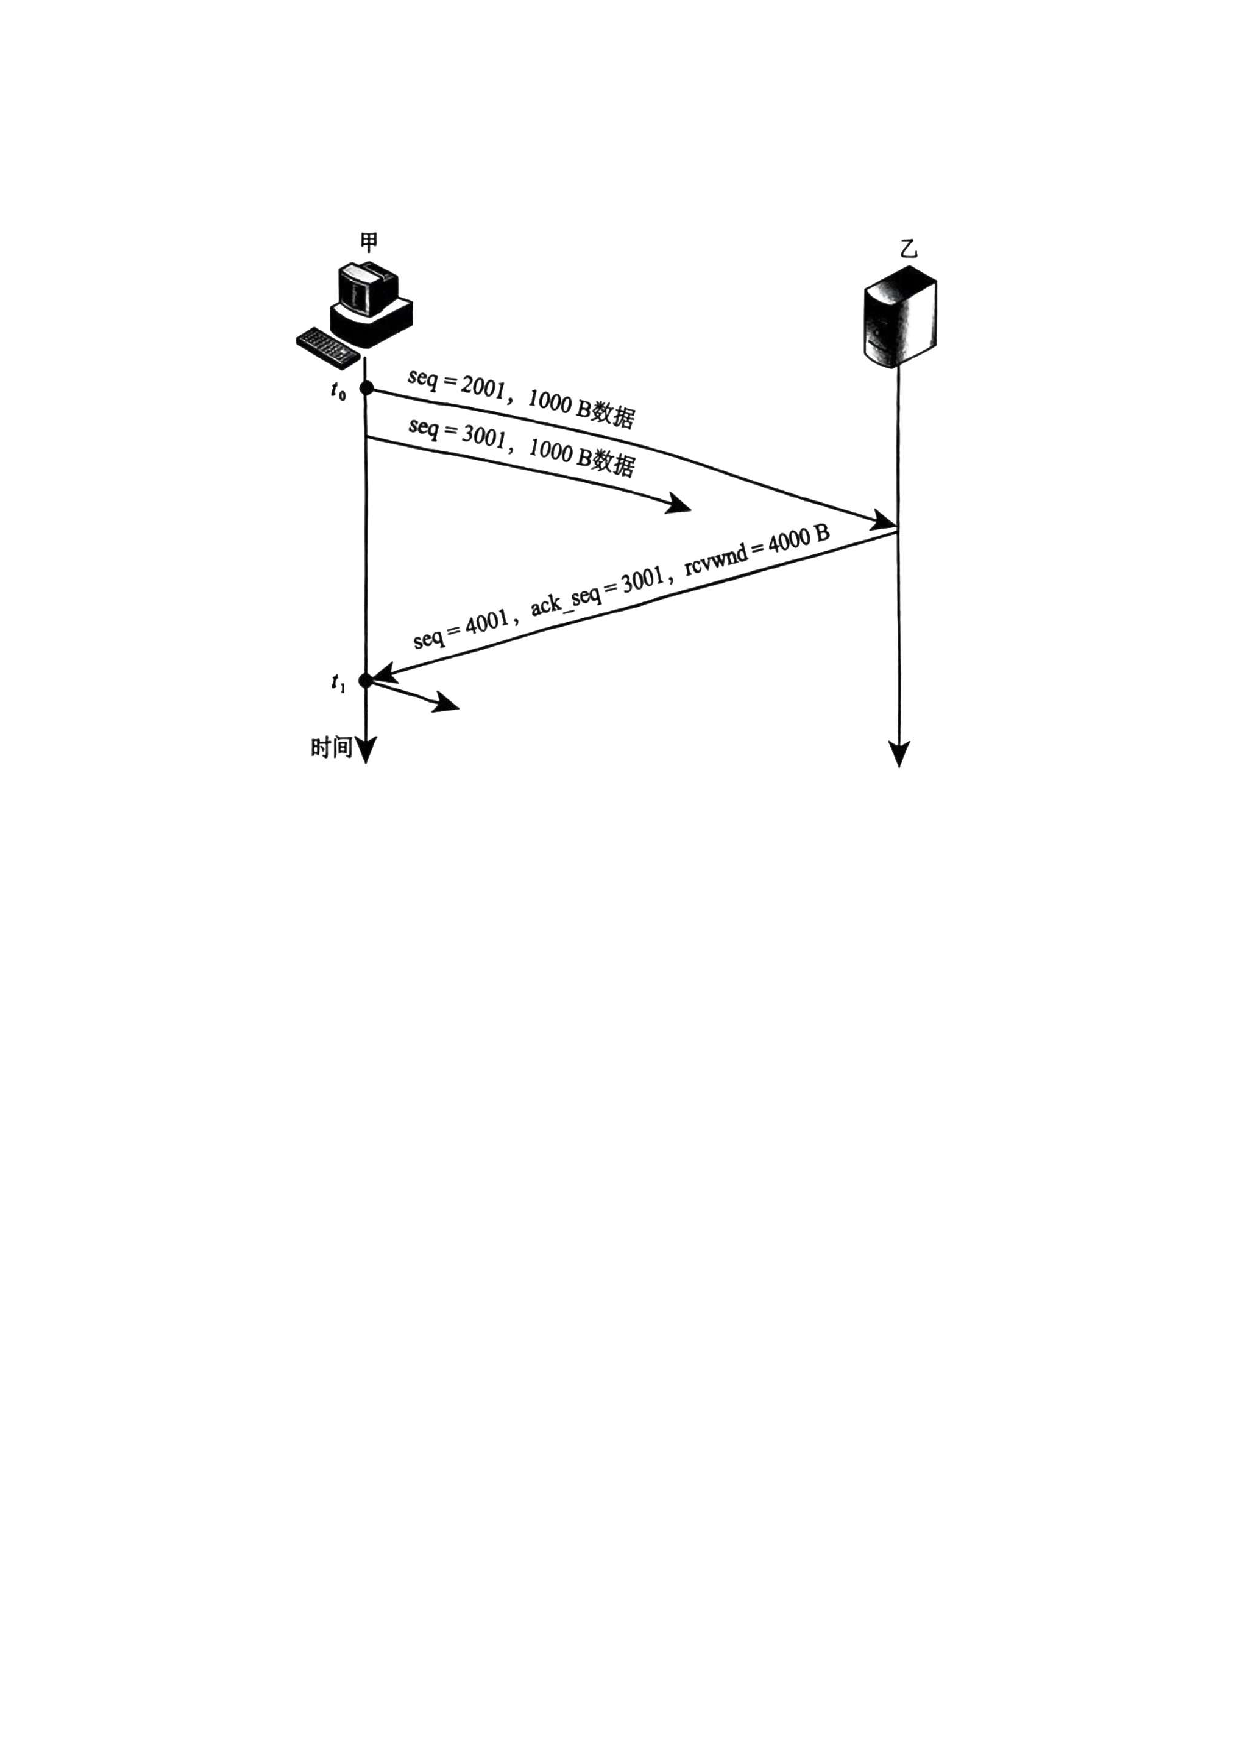
\includegraphics[width=.65\linewidth,height=.4\textheight,keepaspectratio]{../assets/figures/2025-questions-p005-b001.pdf}\end{center}

\begin{center}\begin{tabular}{>{\raggedright\arraybackslash}p{\dimexpr(\linewidth-8\tabcolsep)/4\relax}>{\raggedright\arraybackslash}p{\dimexpr(\linewidth-8\tabcolsep)/4\relax}>{\raggedright\arraybackslash}p{\dimexpr(\linewidth-8\tabcolsep)/4\relax}>{\raggedright\arraybackslash}p{\dimexpr(\linewidth-8\tabcolsep)/4\relax}}
\textbf{A.} 2 & \textbf{B.} 3 & \textbf{C.} 4 & \textbf{D.} 5\\[.35em]\end{tabular}\end{center}

39．Time 是一个提供时间查询服务的C/S 架构网络应用，支持客户通过UDP 或TCP 向Time 服务器请求时间服务。若某客户与某Time 服务器通信的往返时间RTT=8ms，则该客户分别通过UDP 和 TCP 向该服务器请求服务，所需的最少时间分别是：


\begin{center}\begin{tabular}{>{\raggedright\arraybackslash}p{\dimexpr(\linewidth-8\tabcolsep)/4\relax}>{\raggedright\arraybackslash}p{\dimexpr(\linewidth-8\tabcolsep)/4\relax}>{\raggedright\arraybackslash}p{\dimexpr(\linewidth-8\tabcolsep)/4\relax}>{\raggedright\arraybackslash}p{\dimexpr(\linewidth-8\tabcolsep)/4\relax}}
\textbf{A.} 8ms, 8ms & \textbf{B.} 8ms, 16ms & \textbf{C.} 16ms, 8ms & \textbf{D.} 16ms, 16ms\\[.35em]\end{tabular}\end{center}

40．下列关于POP3 协议的叙述中，正确的是： I. 支持用户代理从邮件服务器读取邮件 II. 支持用户代理向邮件服务器发送邮件 III. 支持邮件服务器之间发送与接收邮件 IV. 支持通过一条TCP 连接收取多封邮件


\begin{center}\begin{tabular}{>{\raggedright\arraybackslash}p{\dimexpr(\linewidth-8\tabcolsep)/4\relax}>{\raggedright\arraybackslash}p{\dimexpr(\linewidth-8\tabcolsep)/4\relax}>{\raggedright\arraybackslash}p{\dimexpr(\linewidth-8\tabcolsep)/4\relax}>{\raggedright\arraybackslash}p{\dimexpr(\linewidth-8\tabcolsep)/4\relax}}
\textbf{A.} 仅I、IV & \textbf{B.} 仅II、III & \textbf{C.} 仅I、II、III & \textbf{D.} 仅I、III、IV\\[.35em]\end{tabular}\end{center}

\subsection*{二、综合应用题（第41～47小题，共70分）}

41．（本题13分）设有两个长度均为\(\displaystyle n\)的一维整型数组A和res，对数组A中的每个元素A[i]，计算A[i]与A[j]（\(\displaystyle 0\le i\le j\le n-1\)）乘积的最大值，并将其保存到res[i]中。例如，若A[]=\{1, 4, –9, 6\}，则得到res[]=\{6, 24, 81, 36\}。现给定数组A请设计一个时间和空间上尽可能高效的算法calMulMax，求res中各元素的值。函数原型为：


\begin{Verbatim}[breaklines,breakanywhere,fontsize=\small]
void calMulMax(int A[], int res[], int n)
\end{Verbatim}

要求如下。（1）给出算法的基本设计思想。（4分）（2）根据设计思想，采用C或C++语言描述算法，关键之处给出注释。（7分）（3）说明你所设计算法的时间复杂度和空间复杂度。（2分）


42．（本题10分）某工程包含12个活动，使用题42图所示的AOE网描述，图中各边上标注了活动及其持续时间。


\begin{center}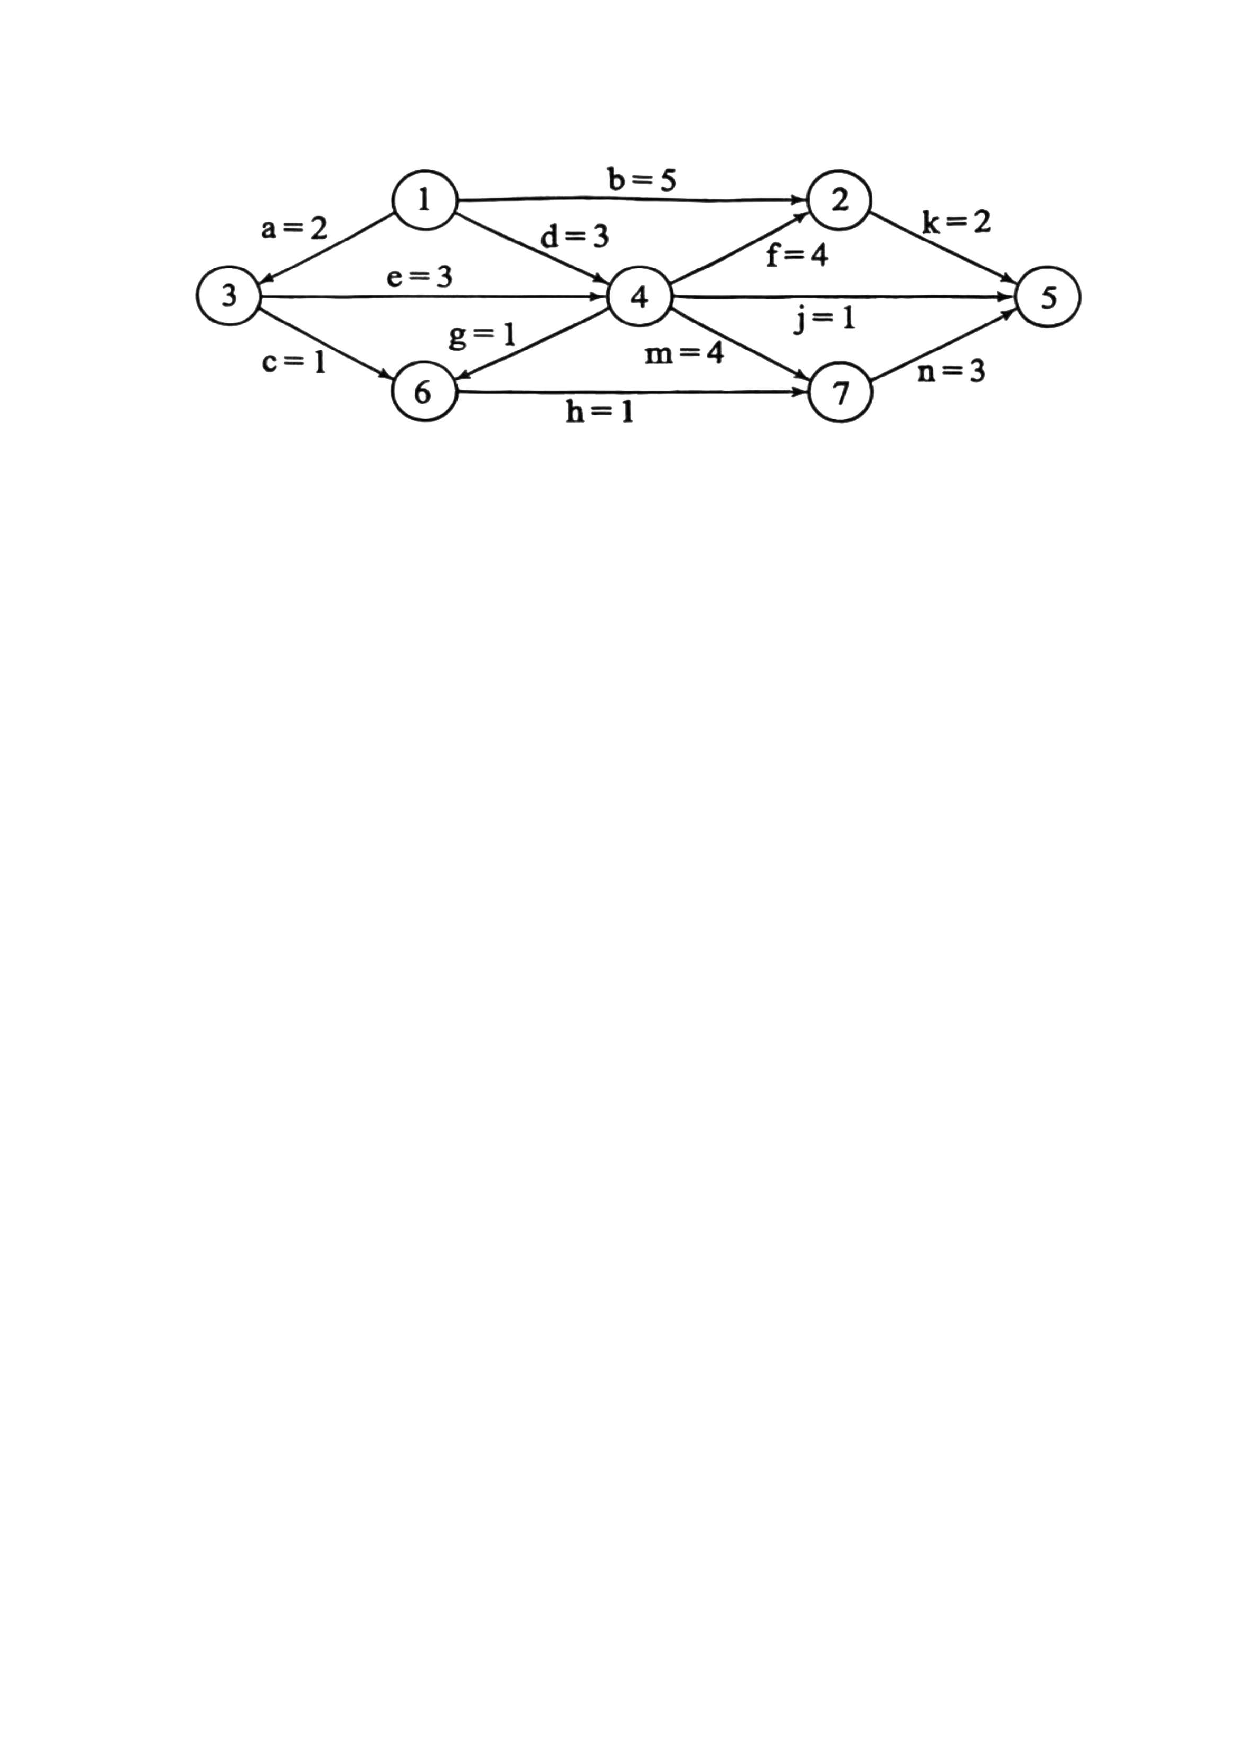
\includegraphics[width=.65\linewidth,height=.4\textheight,keepaspectratio]{../assets/figures/2025-questions-p007-b001.pdf}\end{center}

请回答下列问题（活动均用活动名表示）。（1）完成该工程的最短时间是多少？哪些活动是关键活动？（3分）（2）若以最短时间完成工程，则与活动e同时进行的活动可能有哪些？（3分）（3）时间余量最大的活动是哪个？其时间余量是多少？（2分）（4）假设工程从时刻0启动，因某种原因，活动b在时刻6开始。为了保证工程不延期，在其他活动持续时间均不变的情况下，b的持续时间最多是多少？若不改变b的持续时间，则压缩哪个活动的持续时间也能保证工程不延期？（2分）


43．（本题12分）现有C语言程序P的部分代码如题43图所示。假定运行程序P的计算机M字长为32位，按字节编址，数据Cache的数据区大小为32KB，采用8路组相联映射方式，主存块大小为64B，Cache的命中时间为2个时钟周期，缺失损失为200个时钟周期；采用页式虚拟存储管理方式，页大小为4KB。数组d的起始虚拟地址\(\displaystyle \mathrm{VA}_{31}\sim\mathrm{VA}_{0}\)，为0180 0020H。


\begin{Verbatim}[breaklines,breakanywhere,fontsize=\small]
int x, d[2048], i;
...
for(i=0; i<2048; i++)
  d[i]=d[i]/x;
...
\end{Verbatim}

请回答下列问题。（1）主存地址中Cache组号字段和块内地址字段分别占几位？虚拟地址中哪些位可作为Cache索引？（3分）（2）d[100]的虚拟地址为多少？d[100]所在主存块对应的Cache组号是多少？（2分）（3）假定执行for语句时对应代码已在Cache，变量i和x已装入寄存器，数组d已调入主存但不在Cache，则d[0]在其所在主存块内的偏移量是多少（用十六进制表示）？for语句执行过程中，访问数组d的Cache缺失率和数组元素的平均访问时间分别是多少（Cache缺失率的计算结果要求用百分比表示，保留两位小数）？（5分）（4）数组d分布在几个页中？若执行for语句时对应代码已在主存，但数组d还未调入主存，则执行for语句过程中，访问数组d所引起的缺页次数是多少？（2分）


44．（本题11分）对于题43中计算机M和程序P，假定P的部分机器级代码如题44图（a）所示，其中，R0～R4为通用寄存器，SEXT表示按符号扩展；M中补码除法器逻辑结构如题44图（b）所示。


\begin{Verbatim}[breaklines,breakanywhere,fontsize=\small]
...
//x 在 R2 中，i 在 R4 中
//数组 d 的首地址在 R3 中
mov  R1, (R3+R4*4)  //R1←d[i]
scov R1             //{R0, R1}←SEXT(R1)
idiv R1, R2         //R1←{R0, R1}/R2
...
\end{Verbatim}

\begin{center}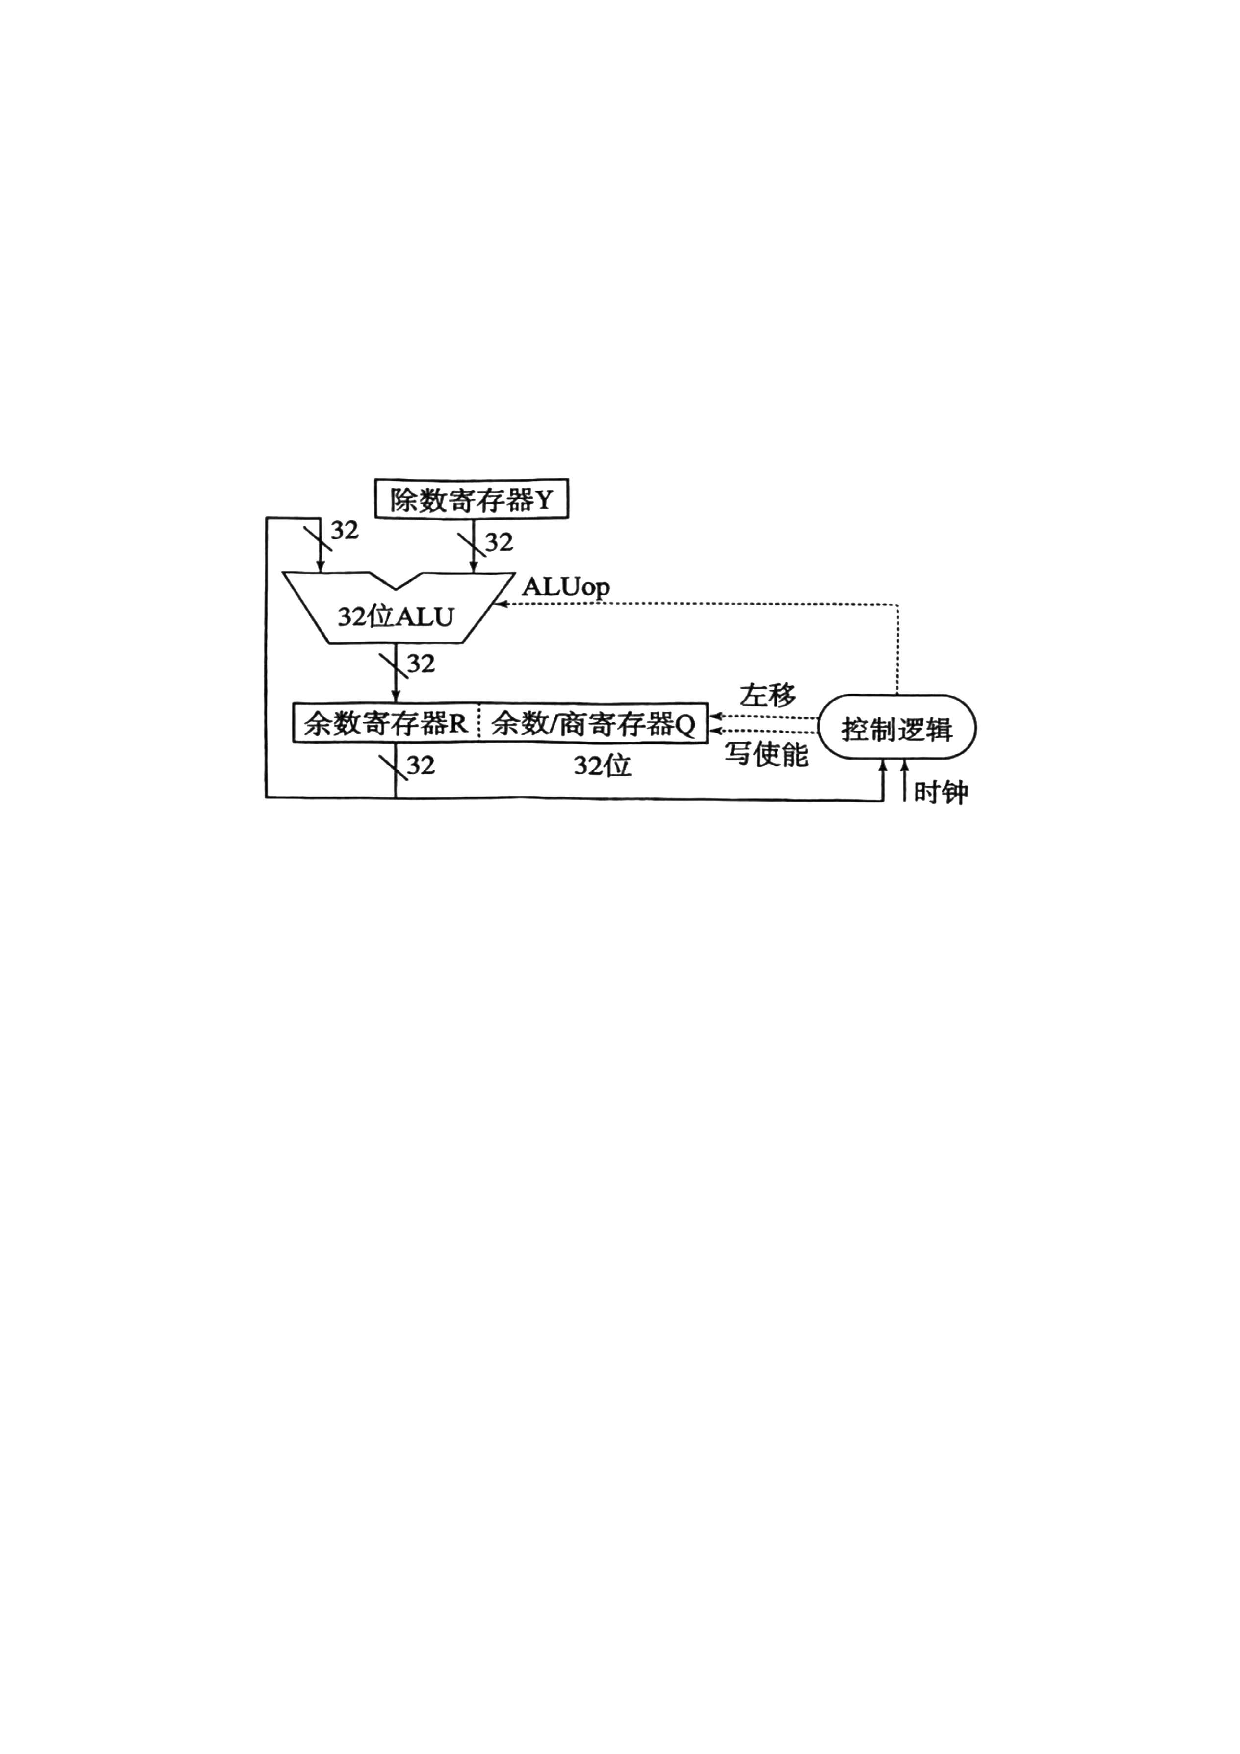
\includegraphics[width=.65\linewidth,height=.4\textheight,keepaspectratio]{../assets/figures/2025-questions-p009-b002.pdf}\end{center}

请回答下列问题。（1）若执行题44图（a）中idiv指令的除运算时，d[i]=0x87654321、x=0xff，则补码除法器中寄存器R、Q和Y的初始内容分别是什么（用十六进制表示）？题44图（b）中哪个部件包含计数器？在补码除法器执行过程中，由ALUop所控制的ALU运算有哪几种？（6分）（2）假设idiv指令执行过程中会检测并触发除法异常，则执行idiv指令时，哪些情况下会发生除法异常（要求给出此时d[i]和x的十六进制表示机器数）？发生除法异常时，在异常响应过程中CPU需要完成哪些操作？（5分）


45．（本题7分）甲、乙、丙三人一起植树，甲负责挖树坑，乙负责将树苗放入树坑中并填土，丙负责为新种的树苗浇水。植树的步骤依次为：挖树坑、放树苗、填土和浇水。现有铁锹和水桶各1个，铁锹用于挖树坑和填土，水桶用于浇水。当树坑的数量小于3时，甲才可以挖树坑。假设初始时树坑的数量为0，铁锹和水桶均可用。请定义尽可能少的信号量，用wait()、signal()操作描述植树过程中三人之间的同步或互斥关系，并说明所用信号量的作用及其初值。


46．（本题8分）某系统中进程的虚拟地址空间包括内核区、用户栈、运行时堆、可读写数据段、只读代码段等区域，其布局如题46图所示，图中阴影部分表示未占用区域。现有C语言程序的部分代码如下。


\begin{Verbatim}[breaklines,breakanywhere,fontsize=\small]
char *ptr;
void main()
{
    int length;
    ptr=(char *)malloc(100);
    scanf("%s", ptr);
    length=strlen(ptr);
    printf("length=%d\n", length);
    free(ptr);
}
\end{Verbatim}

\begin{center}\begin{adjustbox}{max width=\linewidth}\begin{tabular}{|>{\raggedright\arraybackslash}p{\dimexpr(\linewidth-2\tabcolsep-2\arrayrulewidth)/1\relax}|}\hline
虚拟地址空间（由高地址至低地址）\\\hline
内核区\\\hline
用户栈\\\hline
未占用区域（阴影）\\\hline
运行时堆\\\hline
可读写数据段\\\hline
只读代码段\\\hline
未占用区域（阴影）\\\hline\end{tabular}\end{adjustbox}\end{center}

请回答下列问题。（1）上述程序执行时，其进程控制块位于哪个区域？执行scanf()等待键盘输入时，该进程处于什么状态？（2分）（2）main()函数的代码位于哪个区域？其直接调用的哪些函数的功能需要通过执行驱动程序实现？（3分）（3）变量ptr被分配在哪个区域？若变量length没有被分配在寄存器中，则会被分配在哪个区域？ptr指向的字符串位于哪个区域？（3分）


47．（本题9分）某公司在承建国家重大工程项目时，工程部需要较长时间驻扎在偏远山区，工程部网络需要连接公司总部网络。假设综合考虑方案的技术可行性、安全性与经济成本等因素后，决定租用我国自主建设的天通一号卫星通信链路，连接工程部网络的路由器R1和公司总部网络的路由器R2，如题47图所示。S1和S2为千兆以太网交换机；TR1和TR2是卫星信号地面收发设备，实现全双工调制解调。天通一号卫星轨道高度是36 000km，电磁波信号传播速度为300 000km/s。租用的卫星链路为R1和R2之间提供对称全双工信道，每个方向的数据传输速率为200kb/s。


\begin{center}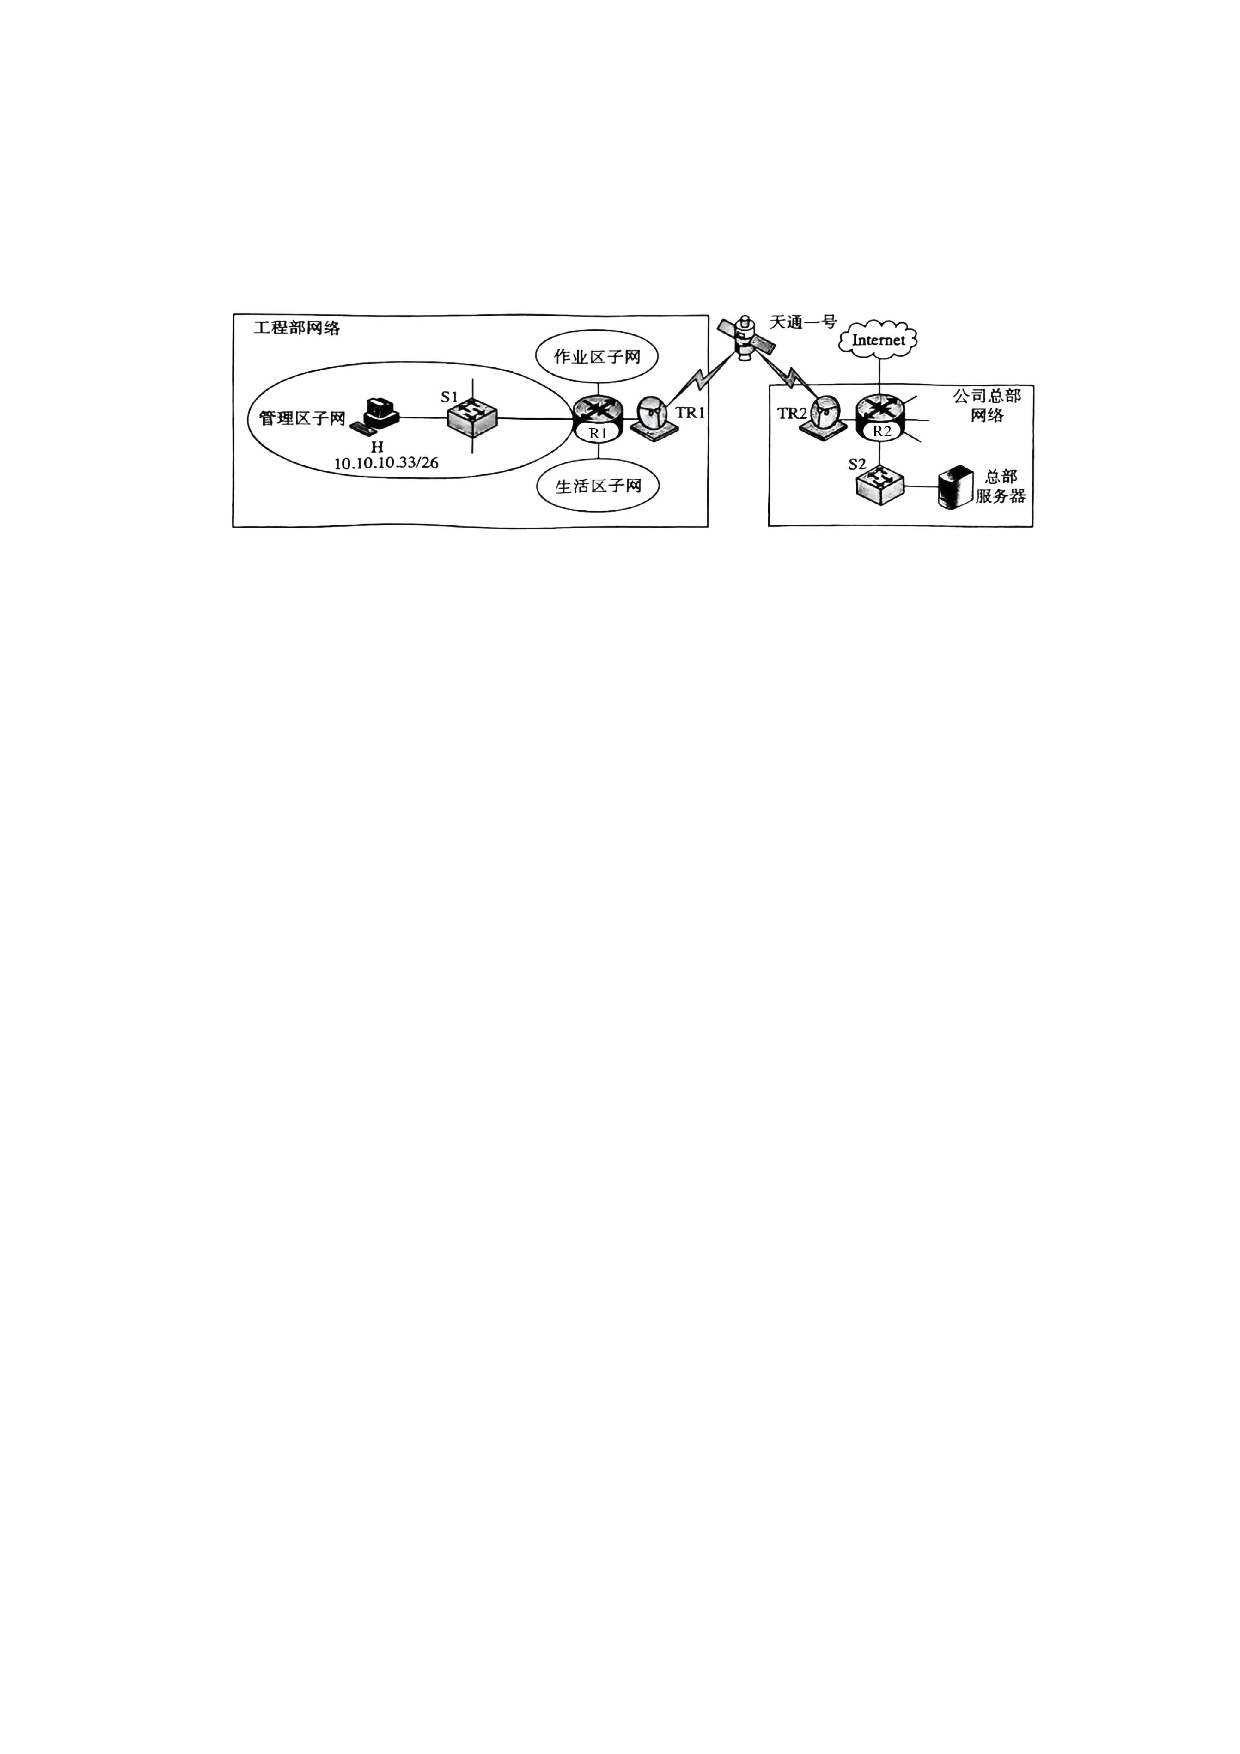
\includegraphics[width=.65\linewidth,height=.4\textheight,keepaspectratio]{../assets/figures/2025-questions-p012-b001.pdf}\end{center}

请回答下列问题。（1）若忽略卫星信号中继以及TR1和TR2调制解调的时间开销，则R1到R2之间卫星链路的单向传播时延是多少？主机H向总部服务器传输数据时可以达到的最大吞吐量是多少？若忽略各层协议数据包的首部开销以及以太网内的传播时延，则主机H向总部服务器上传一个4000B大小的工程进度报告文件，至少需要多长时间？（3分）（2）现需要基于GBN滑动窗口协议为卫星链路设计单向可靠的数据链路层协议SLP，支持R1向R2发送数据，SLP数据帧长为1500B，忽略ACK帧长度。若要求SLP的单向信道利用率不低于80\%，则SLP的发送窗口至少为多少？SLP帧的序号字段至少需要多少位？（3分）（3）若公司总部为工程部网络分配的IP地址空间是10.10.10.0/24，工程部进一步将该IP地址空间分配给3个子网，其中生活区子网可分配IP地址数不少于120个，作业区子网和管理区子网可分配IP地址数均不少于60个，且主机H已正确配置了IP地址，则作业区子网、管理区子网和生活区子网的子网地址分别是什么（给出CIDR地址形式）？（3分）

\end{document}
